\documentclass[pdflatex,compress,mathserif]{beamer}

%\usetheme[dark,framenumber,totalframenumber]{ElektroITK}
\usetheme[darktitle,framenumber,totalframenumber]{ElektroITK}

\usepackage[utf8]{inputenc}
\usepackage[T1]{fontenc}
\usepackage{lmodern}
\usepackage[bahasai]{babel}
\usepackage{amsmath}
\usepackage{amsfonts}
\usepackage{amssymb}
\usepackage{graphicx}
\usepackage{multicol}
\usepackage{lipsum}

\newcommand*{\Scale}[2][4]{\scalebox{#1}{$#2$}}%

\title{PEMODELAN JARINGAN KOMUNIKASI}
\subtitle{Cisco Router and Switch Basics}

\author{Tim Dosen Pengampu}

\begin{document}

\maketitle

\section{Basic Router and Switch Configuration}

\begin{frame}
	\frametitle{Router IP Addresses}
	\begin{itemize}
		\item A router provides connectivity between different IP subnets
		\item An IP address must be configured on the interfaces in each subnet
		\item[] \texttt{interface FastEthernet0/0 \\
			ip address 192.168.0.1 255.255.255.0 \\
			no shutdown \\
			! \\
			interface FastEthernet0/1 \\
			ip address 192.168.1.1 255.255.255.0 \\
			no shutdown}
	\end{itemize}
	\begin{center}
		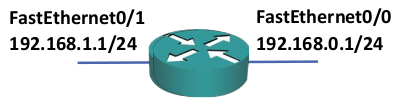
\includegraphics[width=0.4\linewidth]{img/img01}
	\end{center}
\end{frame}

\begin{frame}
	\frametitle{Switch Management IP Address}
	\begin{itemize}
		\item A Layer 2 Switch is not IP routing aware.
		\item It does however support a single IP address for management.
		\item The IP address and subnet mask is configured on the Switched Virtual Interface (SVI) for the default VLAN 1
		\item A default gateway also needs to be configured to allow connectivity to other subnets
	\end{itemize}
\end{frame}



\begin{frame}
	\frametitle{Management IP Address}
	\begin{itemize}
		\item[] \texttt{\scriptsize Switch(config)\# interface vlan 1 \\
			Switch(config-if)\# ip address 192.168.0.10 255.255.255.0 \\
			Switch(config-if)\# no shutdown \\
			Switch(config-if)\# exit \\
			Switch(config)\# ip default-gateway 192.168.0.1}
		\item Additional commands need to be entered to allow Telnet or SSH (Secure Shell) access, we'll cover these in the 'Securing Cisco Devices' section
	\end{itemize}
\end{frame}

\begin{frame}
	\frametitle{Lab Example}
	\begin{center}
		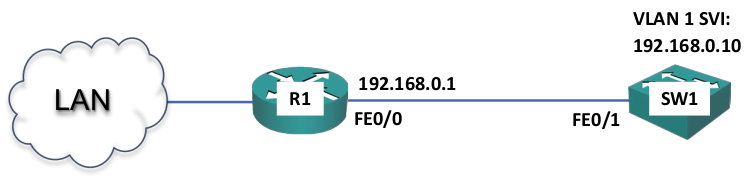
\includegraphics[width=\linewidth]{img/img02}
	\end{center}
\end{frame}

\begin{frame}
	\frametitle{Hostname}
	\begin{itemize}
		\item A descriptive hostname makes it easier to identify the device.
		\item Eg. NY-F1-SW1
		\item[]
		\item[] \texttt{\scriptsize Switch(config)\# hostname SW1\\
			SW1(config)\#}
	\end{itemize}
\end{frame}

\begin{frame}
	\frametitle{Interface Descriptions}
	\begin{itemize}
		\item Interface descriptions can aid troubleshooting
		\item[]
		\item[] \texttt{\scriptsize SW1(config)\# interface FastEthernet 0/1\\
			SW1(config-if)\# description Link to R1}
	\end{itemize}
\end{frame}

\section{Speed and Duplex Settings}

\begin{frame}
	\frametitle{Interface Speed and Duplex}
	\begin{itemize}
		\item Interface speed and duplex is set to 'auto' by default
		\item Both sides of a link should auto-negotiate to full duplex and the fastest available speed
		\item Best practice is to manually set the speed and duplex on ports which are connected to another network infrastructure device or server
		\item It is very important to set matching speed and duplex settings on both sides of the link
	\end{itemize}
\end{frame}

\begin{frame}{Interface Speed and Duplex}
	\texttt{SW1(config)\# interface FastEthernet 0/1 \\
		SW1(config-if)\# duplex full \\
		SW1(config-if)\# speed 100}
\end{frame}

\begin{frame}
	\frametitle{Verification Commands}
	\texttt{SW1\# show running-config \\
	SW1\# show ip interface brief \\
	SW1\# show run interface vlan 1 \\
	SW1\# show interface vlan 1 \\
	SW1\# show version \\}
\end{frame}

\section{CDP and LLDP}

\begin{frame}
	\frametitle{CDP Cisco Discovery Protocol}
	\begin{itemize}
		\item Cisco Discovery Protocol (CDP) is a Cisco proprietary Layer 2 protocol.
		\item It is used to share information with other directly connected Cisco equipment, such as the operating system version and IP address.
		\item This aids in troubleshooting by allowing administrators to map out how Cisco devices are connected to each other.
		\item It is enabled by default on most Cisco equipment.
		\item It works at Layer 2 so it is not necessary for the device to have an IP address.
	\end{itemize}
\end{frame}

\begin{frame}{CDP Cisco Discovery Protocol}
	\texttt{Switch(config)\# cdp run \\
		Switch(config)\# no cdp run \\
		Switch(config-if)\# no cdp enable \\
		Switch\# show cdp \\
		Switch\# show cdp neighbors \\
		Switch\# show cdp neighbors detail \\}
\end{frame}

\begin{frame}
	\frametitle{LLDP Link Layer Discovery Protocol}
	\begin{itemize}
		\item LLDP (Link Layer Discovery Protocol) is an open standard protocol which provides similar information to CDP.
		\item Differences with CDP:
		\begin{itemize}
			\item Depending on the switch and version it may be disabled by default
			\item It is only supported on physical interfaces
			\item It can only discover up to one device per port
			\item It can discover Linux servers
		\end{itemize}		
	\end{itemize}
\end{frame}

\begin{frame}
	\frametitle{LLDP Link Layer Discovery Protocol\\ Configuration}
	\texttt{Switch(config)\# lldp run \\
		Switch(config)\# no lldp run \\
		Switch(config-if)\# no lldp transmit \\
		Switch(config-if)\# no lldp receive \\
		Switch\# show lldp \\
		Switch\# show lldp neighbors \\
		Switch\# show lldp neighbors detail \\}
\end{frame}

\section{Basic Layer 1 and Layer 2 Troubleshooting}

\begin{frame}
	\frametitle{Layer 1 Troubleshooting}
	\begin{itemize}
		\item Basic switch troubleshooting involves checking for Layer 1 and Layer 2 issues
		\item Copper and Fibre cables are liable to break if not handled correctly
	\end{itemize}
\end{frame}

\begin{frame}{Layer 1 Troubleshooting}
	\begin{itemize}
		\item Common Layer 1 problems include:
		\begin{itemize}
			\item The interface is administratively shut down
			\item The cable is disconnected on either or both ends
			\item The device on the other end of the cable is powered off
			\item Broken connectors which cause loose connections
			\item Bent or stretched cables which lead to broken wires or fibres
			\item Electro-Magnetic Interference (EMI) sources such as motors or microwaves which cause errors in transmission (newer cable is less susceptible to this)
		\end{itemize}
	\end{itemize}
\end{frame}

\begin{frame}
	\frametitle{Layer 1 Troubleshooting Commands}
	\texttt{Switch\# show ip interface brief}
	\begin{itemize}
		\item 'administratively down' – Issue 'no shutdown'
		\item 'down/down' – This indicates a Layer 1 issue. Check the interface is cabled at both ends and the device on the other side is powered on
		\item 'up/down' – This indicates a Layer 2 issue or speed mismatch. Check the interface configuration matches on both sides of the link
	\end{itemize}
\end{frame}

\begin{frame}
	\frametitle{Show ip interface brief}
	\begin{center}
		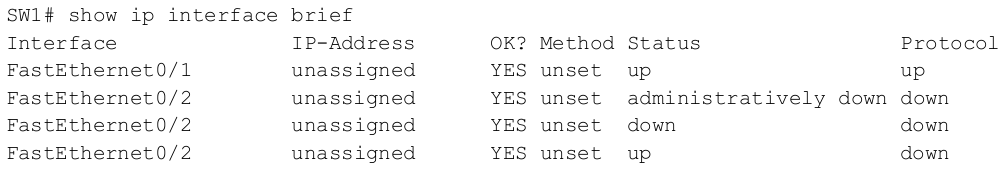
\includegraphics[width=\linewidth]{img/img03}
	\end{center}
\end{frame}

\begin{frame}
	\frametitle{Show Interface}
	\texttt{Switch\# show interface}
	\begin{itemize}
		\item If the interface is reporting an excessive amount of errors it could be either a Layer 1 or Layer 2 problem
		\item Check the integrity of the cable
		\item Check the configuration matches on both sides of the link
	\end{itemize}
\end{frame}

\begin{frame}{Show Interface}
	\begin{center}
		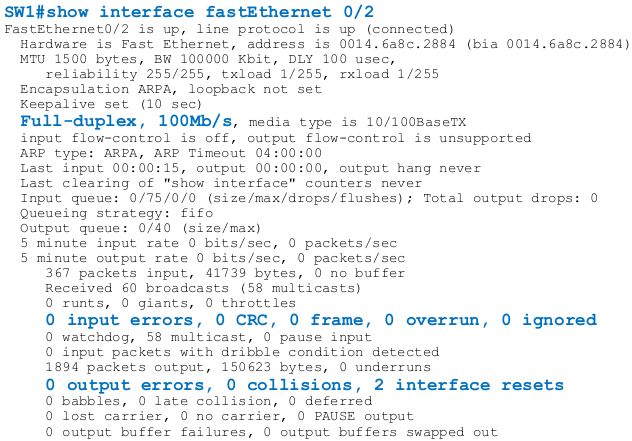
\includegraphics[width=0.8\linewidth]{img/img04}
	\end{center}
\end{frame}

\begin{frame}
	\frametitle{Speed and Duplex Mismatches}
	\begin{itemize}
		\item A possible error is speed and/or duplex mismatches
		\item Incorrect speed settings can cause the interface to operate below its maximum speed
		\item Speed mismatches will typically bring the interface down
		\item The interface will typically stay up with duplex mismatches but performance will be terrible because of collisions
		\item The \texttt{show interface} command will report an excessively high number of errors in this case
	\end{itemize}
\end{frame}

\begin{frame}{Speed and Duplex Mismatches}
	\begin{itemize}
		\item Both sides of a link must be set the same, as either auto or manually configured
		\item Cisco devices default to auto
		\item If one side is set to auto, and the other is manually configured, this will often result in a mismatch
		\item Best practice is to manually configure ports attached to other network infrastructure devices or servers
		\item Remember to manually configure both sides of the link!
		\item If a device has issues with auto negotiating speed or duplex, manually configuring both sides will normally solve the problem
	\end{itemize}
\end{frame}

\begin{frame}
	\frametitle{Speed and Duplex Mismatches - CDP}
	\begin{itemize}
		\item CDP should detect a duplex mismatch
		\item[] \texttt{\%CDP-4-DUPLEX\_MISMATCH: duplex mismatch discovered on FastEthernet0/0 (not half duplex)}
	\end{itemize}
\end{frame}

\end{document}
